\documentclass[../report.tex]{subfiles}


\begin{document}
\graphicspath{{img/}{../img/}}

\section*{Target project}
For this paper we will study the project carried out by ourselves for the ITU course 
Second Year Project: Software Development in Large Teams with International Collaboration.
In the target project we are to collaborate with a team of students from Singapore Management University
developing a computer system for uploading and downloading resources. The system will have two
individual front-ends with a shared back-end. In addition we are required to document the design
of the system as well as our collaboration with the Singaporean students.

\section*{Problem statement}
In this paper we aim to answer the following question in regards to the target project.
\newline	
\textbf{How can you plan and execute an exam project like the target project well?}
\begin{itemize}
	\item	How can you estimate the time required for each of the subtasks of the target project?
	\item 	How can you balance estimated time with available time to reach a satisfying product by the set deadline?
	\item 	How can you choose a fitting process model for the target project?
	%\item 	How can you manage resources and keep the target project on track?
	\item 	Which parts of the target project could have been done differently for a better result?
\end{itemize}

\section*{Method}
%To answer the problem statement we will look at the tools used in the target project. Additionally we will apply other tools to the target project and evaluate the different results. Using these tools include doing calculations and creating diagrams.

To answer the problem statement we will look at different methodologies for estimating, planning and executing activities in the target project. In the target project we will apply the Delphi method for estimating activities, a simplified version of SCRUM (Scrum-but) as a process model and a Gantt chart for planning the activities. Additionally we will consider but not apply alternative methods for comparison. This includes Function Points for estimating activities, The Waterfall Model and The Spiral Model as process models and The Precedence Network for planning activities. 

%Forskellige estimeringsmetoder: FP, Delphi
%Forskellige processmodeller: Vandfald, SCRUM, spiral
%Forskellige aktivitetsplanl�gningsmetoder: precedence network (critical path), gantt


\newpage
\newgeometry{left=7cm,bottom=0.1cm}
\begin{landscape}

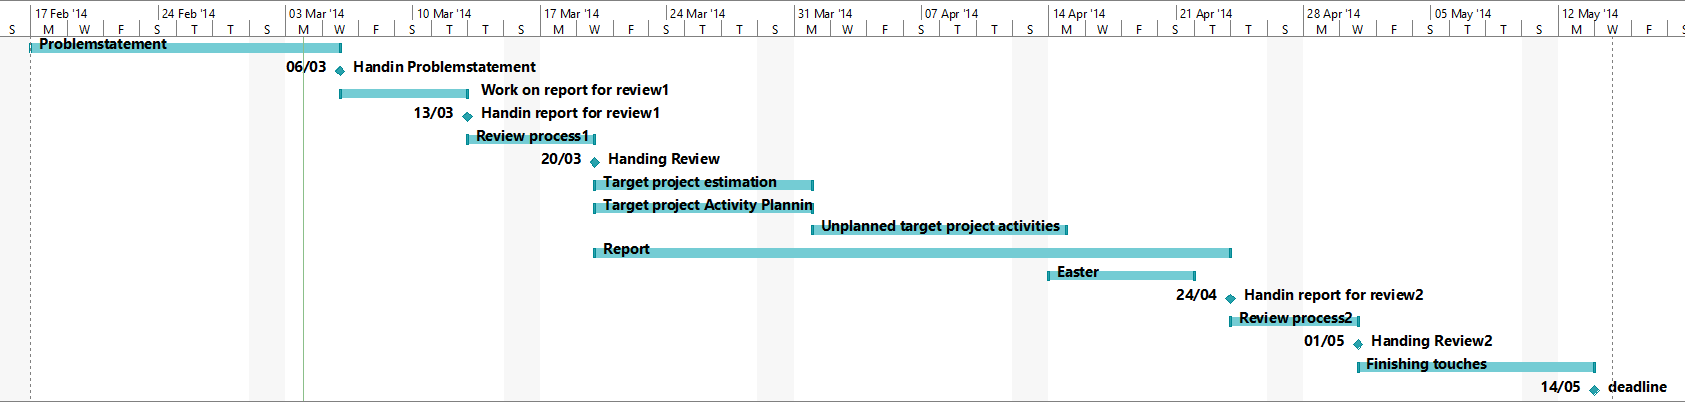
\includegraphics[ scale=0.6]{timeschedule.png}


\end{landscape}




\end{document}
